\documentclass{standalone}
\usepackage{tikz}

\definecolor{colstraat}{HTML}{bcc2c2}
\definecolor{colfietspad}{HTML}{eda596}
\definecolor{colvoetpad}{HTML}{727878}

\begin{document}


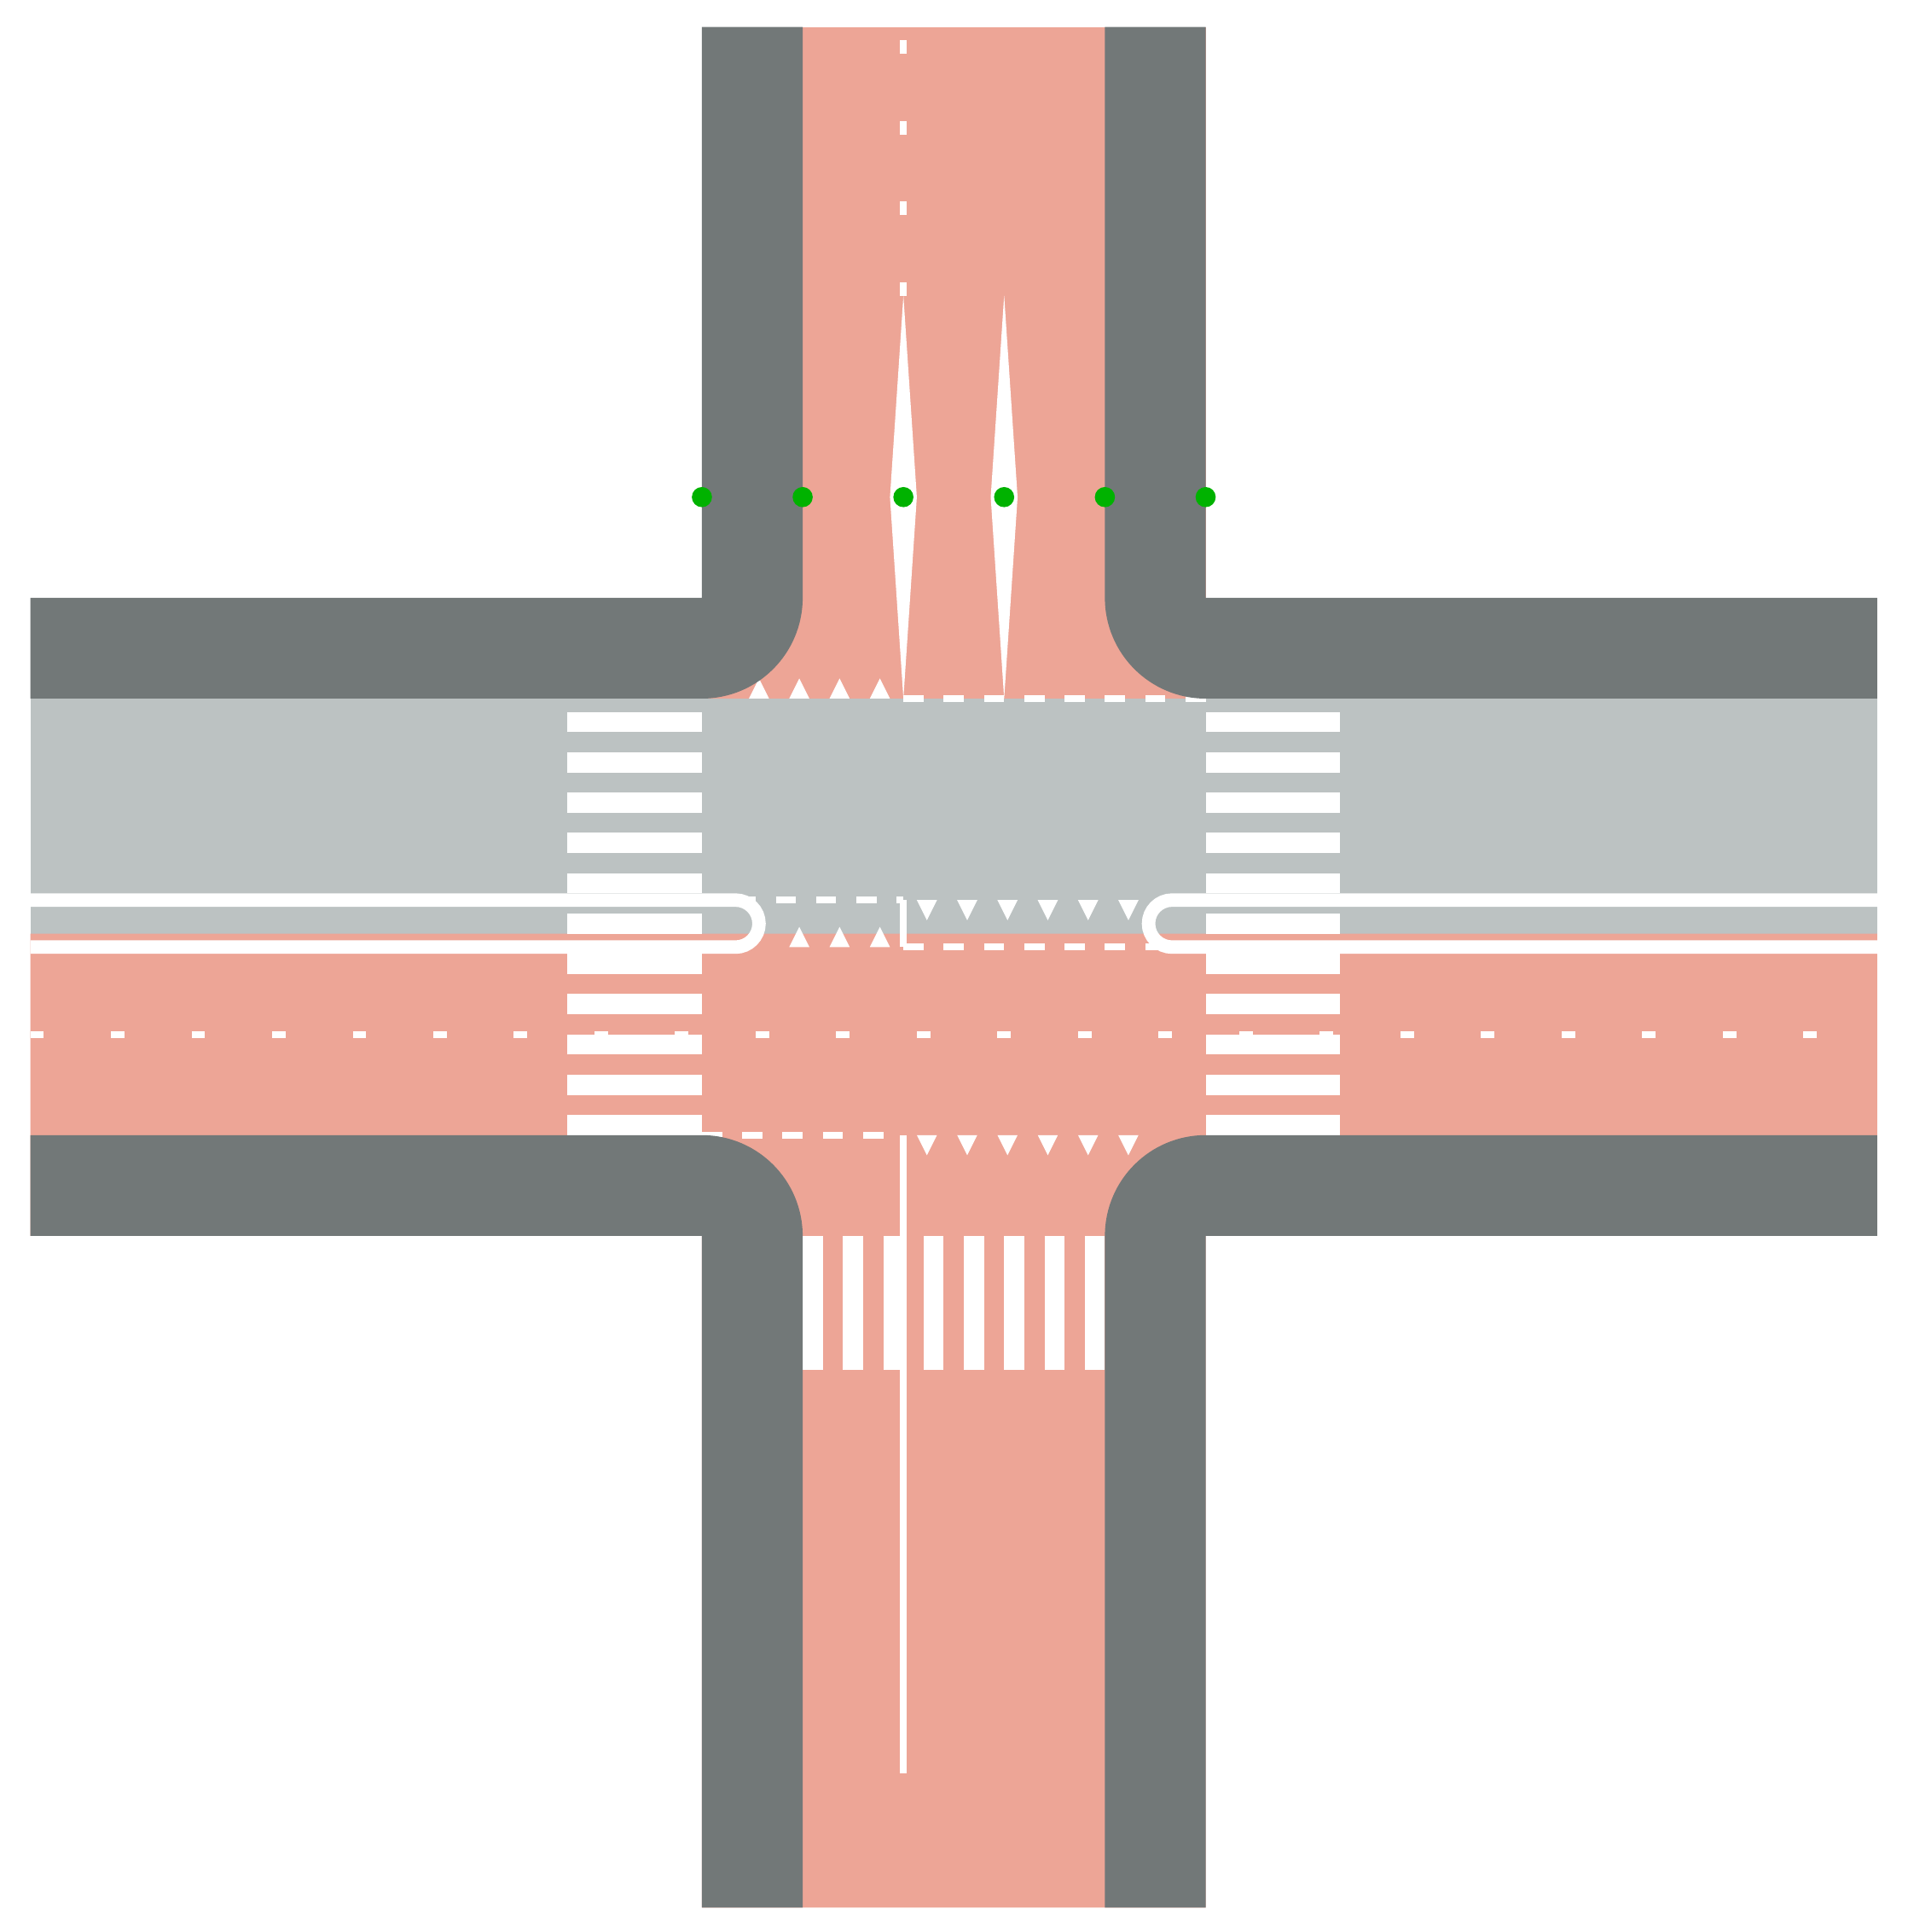
\begin{tikzpicture}
%%% straat
\fill[colstraat] (0,14.5) rectangle (27.5,18);
%%% fietsweg
\fill[colfietspad] (0,14.5) -- (0,10) -- (10,10) -- (10,0) -- (17.5,0) -- (17.5,10) -- (27.5,10) -- (27.5,14.5) -- cycle;
\fill[colfietspad] (10,18) rectangle (17.5,28) ;
%%% lijnen
\draw[white,line width=1mm] (13,11.5) -- (13,2);
\draw[white,line width=1mm,dash pattern=on .3cm off .3cm] (10,11.5) -- (13,11.5);
\foreach \x in {13.2,13.8,14.4,15.0,15.6,16.2}{
	\fill[white] (\x,11.5) -- +(.3,0) -- +(.15,-.3) -- cycle; 
	}
\draw[white,line width=1mm,dash pattern=on 2mm off 1cm] (0,13) -- (27.5,13);
\draw[white,line width=2mm] (0,14.3) -- (10.5,14.3) arc[start angle=270,delta angle=180,radius=.35] -- (0,15) ;
\draw[white,line width=2mm] (27.5,14.3) -- (17,14.3) arc[start angle=270,delta angle=-180,radius=.35] -- (27.5,15) ;
\draw[white,line width=1mm] (13,14.3) -- (13,15);
\foreach \x in {13.2,13.8,14.4,15.0,15.6,16.2}{
	\fill[white] (\x,15) -- +(.3,0) -- +(.15,-.3) -- cycle; 
	}
\foreach \x in {12.8,12.2,11.6}{
	\fill[white] (\x,14.3) -- +(-.3,0) -- +(-.15,.3) -- cycle; 
	}
\draw[white,line width=1mm,dash pattern=on .3cm off .3cm] (10.5,15) -- (13,15);	
\draw[white,line width=1mm,dash pattern=on .3cm off .3cm] (13,14.3) -- (17.5,14.3);	
	
\fill[white] (13,18) -- +(-.2,3) -- +(0,6) -- +(.2,3) -- cycle;
\draw[white,line width=1mm,dash pattern=on 2mm off 1cm] (13,24) -- (13,28);
\fill[white] (14.5,18) -- +(-.2,3) -- +(0,6) -- +(.2,3) -- cycle;
\foreach \x in {12.8,12.2,11.6,11.0}{
	\fill[white] (\x,18) -- +(-.3,0) -- +(-.15,.3) -- cycle; 
	}
\draw[white,line width=1mm,dash pattern=on .3cm off .3cm] (13,18) -- (17.5,18);
%%% zebrapaden
\draw[white,line width=2cm,dash pattern=on .3cm off .3cm] (11.5,9) -- (16,9);
\draw[white,line width=2cm,dash pattern=on .3cm off .3cm] (9,11.5) -- (9,18);
\draw[white,line width=2cm,dash pattern=on .3cm off .3cm] (18.5,11.5) -- (18.5,18);

%%% voetpaden
\fill[colvoetpad] (11.5,0) -- (11.5,10) arc[start angle=0,delta angle=90,radius=1.5] -- (0,11.5) --(0,10) -- (10,10) -- (10,0) -- cycle;
\fill[colvoetpad] (16,0) -- (16,10) arc[start angle=180,delta angle=-90,radius=1.5] -- (27.5,11.5) --(27.5,10) -- (17.5,10) -- (17.5,0) -- cycle;
\fill[colvoetpad] (11.5,28) -- (11.5,19.5) arc[start angle=0,delta angle=-90,radius=1.5] -- (0,18) --(0,19.5) -- (10,19.5) -- (10,28) -- cycle;
\fill[colvoetpad] (16,28) -- (16,19.5) arc[start angle=180,delta angle=90,radius=1.5] -- (27.5,18) --(27.5,19.5) -- (17.5,19.5) -- (17.5,28) -- cycle;
%%% paaltjes
\foreach \x in {10,11.5,13,14.5,16,17.5}{
	\fill[green!70!black] (\x,21) circle (.15cm);
	}



%%%% GRID
%\draw[step=1cm,pink,very thin] (0,0) grid (28,28);
%\foreach \i in {1,...,28}{
%	\node[blue] at (\i,0) [anchor=north]{\i};
%	\node[blue] at (0,\i) [anchor=east]{\i};
%	}
\end{tikzpicture}







\end{document}
